\documentclass{jfm}

% Compilation
\usepackage{silence} % Silence latex compiler warnings
\WarningFilter{latex}{Command \@xhline has changed} % Filter out warning
  % caused by redefinition between jfm.cls class and array (loaded by
  % siunitx)

% Import custom style file containing common packages and options
\setlength{\paperheight}{\pdfpageheight} % JFM class removes paperheight definition and hyperref raises a warning

% Import custom style file containing common packages and options
\usepackage{preamble}
\graphicspath{{./Figures/}}

% Discrete Fourier Transform
\newcommand{\GenP}{\hat{P}_m}
\newcommand{\POne}{\hat{P}_1}
\newcommand{\PTwo}{\hat{P}_2}
\newcommand{\PThree}{\hat{P}_3}
\newcommand{\PFour}{\hat{P}_4}

% Continuous Fourier Transform
\newcommand{\GenPk}{\hat{P} (\kappa)}
\newcommand{\PZerok}{\hat{P} (0)}

% Define custom math symbols
\DeclareMathOperator{\cn}{Cn}
\DeclareMathOperator{\sgn}{sgn}
\DeclareMathOperator{\Ur}{Ur}
\DeclareMathOperator{\Sk}{Sk}
\DeclareMathOperator{\As}{As}
%\DeclareMathOperator{\Bi}{Bi}

\newcommand{\hilbert}{\mathcal{H}}

% Define custom math functions
\DeclarePairedDelimiter{\round}{\lfloor}{\rceil}

% Define \im as Roman i
\newcommand{\im}{\mathrm{i}}
% Replace epsilon with varepsilon
\renewcommand*{\epsilon}{\varepsilon}

%% Use \thalf and \squart commands from JFM class
%\newcommand\squart{\ensuremath{{\textstyle\frac{1}{4}}}}
%\newcommand\thalf{\ensuremath{{\textstyle\frac{1}{2}}}}

\linenumbers{}

\title{Wind-Induced Changes to Surface Gravity Wave Shape in Shallow Water}

\author{Thomas J. Zdyrski \and Falk Feddersen}

\begin{document}

\maketitle

\begin{abstract}
Wave shape (\eg{} wave skewness and asymmetry) impacts sediment
transport, remote sensing and ship safety.
Previous work by the authors showed that wind (via changes in surface
pressure) affects wave shape in intermediate and deep water.
This effect was most pronounced as the depth decreased.
The current work investigates the interaction of wind and wave shape in
shallow water.
A multiple-scales analysis of long waves propagating over a shallow,
flat bottom and forced by a Jeffreys-type surface pressure produces a
Korteweg-de Vries (KdV)-Burgers equation governing the wave profile.
The evolution of an initially symmetric solitary wave is calculated
numerically.
The wave's height, skewness and asymmetry are investigated as functions
of time and pressure magnitude.
These results are in qualitative agreement with prior results in
intermediate and deep water.
\end{abstract}

\section{Introduction}

The study of wind's interaction with ocean waves has a long history, beginning
with \citet{jeffreys1925formation}, and continues to be an active field
of
research~\citep[\eg][]{janssen1991quasi,donelan2004limiting,sulivan2010dynamics}.
Many theoretical
studies~\citep[\eg][]{jeffreys1925formation,miles1957generation,phillips1957generation}
focus on calculating wind-induced growth rates and often employed a
phase-averaging technique.
However, it is also known that wind can influence wave
shape~\citep[\eg][]{leykin1995asymmetry,feddersen2005wind,zdyrski2020wind},
which can be represented by third-order shape statistics such as
skewness and asymmetry, corresponding to the wave's vertical and
horizontal asymmetry, respectively.
Wave shape influences sediment transport
\citep[\eg][]{drake2001discrete, gonzalez2007seabed} which modulates
beach morphodynamics~\citep[\eg][]{hoefel2003wave}.
Additionally, wave skewness affects the returned signal in radar
altimetry~\citep[\eg][]{hayne1980radar,huang1983non},
and wave asymmetry influences ship response to wave
impacts~\citep[\eg][]{soares2008abnormal,oberhagemann2013prediction}.
Therefore, understanding how wind influences these shape statistics is a
matter of practical importance.

When the water depth $h$ is small compared to the wavelength $\lambda$,
waves are classified as shallow-water waves $kh \ll 1$ (with $k
\coloneqq 2 \pi/\lambda$).
Waves in shallow water differ qualitatively from those in intermediate
to deep water where $kh \sim 1$ or $\gg 1$, respectively.
For waves with amplitudes $a_0$ much less than the water depth $h$,
leveraging the small parameters $a/h \sim (kh)^2 \ll 1$
yields the Boussinesq equations for small waves in shallow water.
The waves' interactions with the bottom modifies the dispersion
relation, causes shallow-water wave trains to be weakly dispersive and
permits a special class of waves wherein dispersion balances nonlinear
focusing known as solitary waves.
These have appeared in environments ranging from nonlinear optical pulses
\citep[\eg][]{kivshar1993dark} to astrophysical dusty plasmas
\citep[\eg][]{sahu2012nonextensive}.
One of the simplest models for solitons is the Korteweg-de Vries (KdV)
equation, which incorporates dispersion and nonlinearity.
When augmented with a dissipative term, this becomes the KdV-Burgers
equation.
The KdV-Burgers equation appears across disciplines including damped
internal tides \citep[\eg][]{sandstrom1995dissipation}, electron waves
in graphene \citep[\eg][]{zdyrski2019effects} and viscous flow in blood
vessels \citep[\eg][]{antar1999weakly}.
In order to investigate the interaction of wind and surface waves in
shallow water, we introduce a wind-induced pressure term in the
Boussinesq equations in \cref{sec:derivation}.
This will produce a KdV-Burgers equation governing the surface profile's
evolution, which we will solve numerically.
We analyze the wave height, skewness and asymmetry in
\cref{sec:results}.
Finally, we discuss wind speeds and compare the results to intermediate
and deep-water waves in \cref{sec:discussion}.

\section{\label{sec:derivation} Derivation of KdV-Burgers Equation}

\subsection{Governing Equations}
We will treat the flow as irrotational and inviscid throughout the
fluid and neglect surface tension by restricting to characteristic
length scales much greater than \SI{2}{\centi\meter}.
Furthermore, we restrict to planar wave propagation in the $+x$
direction.
Finally, we choose a coordinate system with $z=0$ at the mean water
level and a horizontal, flat bottom located at $z=-h$.
Then, the incompressibility condition and standard boundary conditions
are
\begin{alignat}{2}
  0 &= \phi_{xx} + \phi_{zz} &&\qq{on}
  -h < z < \eta \,, \label{eq:laplace}\\
  0 &= \phi_{z} &&\qq{on} z=-h \,, \label{eq:bottom_bc}\\
  \phi_{z} &= \eta_{t} + \phi_{x} \eta_{x} &&\qq{on} z = \eta \,,
  \label{eq:kinematic_bc}\\
  \qq*{and} 0 &= \frac{p}{\rho_w} + g\eta + \phi_{t} +
  \frac{1}{2} \bqty{\phi_{x}^2 + \phi_{z}^2} &&\qq{on} z=
  \eta \,. \label{eq:dynamic_bc}
\end{alignat}
Here, $\eta(x,t)$ is the wave profile, $\phi(x,z,t)$ is the flow
velocity potential related to the velocity $\vec{u} = \grad{\phi}$,
$p(x,t)$ is the surface pressure, $g$ is the acceleration due to
gravity and $\rho_w$ is the water density.
We also used the gauge freedom in the definition of $\phi$ to absorb the
Bernoulli `constant' $C(t)$ in the dynamic boundary condition.
We are seeking a solitary, progressive wave which decays at infinity,
\begin{gather}
  \eta(\vec{x},t) \to 0 \qq{as} \abs{\vec{x}} \to \infty \,,
\end{gather}
with similar conditions on $\vec{u}$.
We will choose a coordinate system where the average bottom horizontal
velocity vanishes:
\begin{equation}
  \overline{ \pdv{\phi}{x} } = 0 \qq{on} z=-h \,,
  \label{eq:bot_bc_horz}
\end{equation}
with the overline a spatial average $\overline{f} \coloneqq
\lim_{L\to\infty} \int_{-L}^{L} f \dd{x} / (2L)$.
Additionally, we assume the surface pressure $p(x,t)$ is a Jeffreys-type
forcing \citep{jeffreys1925formation}:
\begin{equation}
  p(x,t) = P \pdv{\eta(x,t)}{x} \,.
\end{equation}
Here, $P$ is proportional to $(U-c)^2$, with $c$ the phase speed and $U$
the wind speed (\cf{} \cref{sec:press_mag}), and $P>0$ corresponds to
(`onshore') wind in the same direction as the wave while $P<0$ denotes
(`offshore') wind opposite the wave.
We use a Jeffreys forcing for its analytic simplicity and clear
demonstration of wind-wave coupling.
Though Jeffrey's separated sheltering mechanism is likely only relevant
in special situations (\eg{} near breaking,
\citealp{banner1976separation}, or for steep waves under strong winds,
\citealp{tian2013evolution,touboul2006interaction}),
a fully dynamic coupling between wind and waves---necessary for an
accurate surface pressure---is outside the scope of this paper.

\subsection{\label{sec:nondim} Non-dimensionization}
We will non-dimensionize our system with the known characteristic
scales: the horizontal length scale $L$ over which $\eta$ changes
rapidly, expressed as an effective wavenumber $k_E \coloneqq 2 \pi/L$;
the (initial) wave amplitude $a_0 = H_0/2$ (\ie{} half the wave height
$H_0$); the depth $h$; the gravitational acceleration $g$; and the wind
speed $U$ expressed as a pressure magnitude $P \propto \rho_a (U-c)^2$.
Denoting non-dimension variables with a prime, we have
\begin{equation*}
  \begin{aligned}
  x &= \frac{x'}{k_E} = h \frac{x'}{\sqrt{\mu_E}}\,, \\
  z &= h z' \,,
  \end{aligned}
  \qquad
  \begin{aligned}
  t &= \frac{t'}{k_E\sqrt{g h}}
    = \frac{t'}{\sqrt{\mu_E}} \sqrt{\frac{h}{g}} \,, \\
  P &= \epsilon P' \frac{\rho_w g}{k_E}
    = \frac{\epsilon}{\sqrt{\mu_E}} P' \rho_w g h \,,
  \end{aligned}
  \qquad
  \begin{aligned}
  \eta &= a_0 \eta' = h \epsilon \eta' \,, \\
  \phi &= \phi'\frac{a_0}{k_E}\sqrt{\frac{g}{h}}
    = \frac{\phi'\epsilon}{\sqrt{\mu_E}}\sqrt{g h^3} \,.
  \end{aligned}
\end{equation*}
The dynamics of our system are controlled by three small,
non-dimensional parameters: $\epsilon \coloneqq a_0/h$, $\mu_E \coloneqq
(k_E h)^2$ and $P k_E/(\rho_w g)$.
We will later require $\order{\epsilon} = \order{\mu_E} =
\order{Pk_E/(\rho_w g)}$.
Now, our non-dimension equations take the form
\begin{alignat}{2}
  0 &= \mu_E \phi'_{x'x'} + \phi'_{z'z'} &&\qq{on}
    -1 < z' < \epsilon \eta' \,, \label{eq:laplace_nondim} \\
  0 &= \phi'_{z'} &&\qq{on} z'=-1 \,, \label{eq:bottom_bc_nondim} \\
  \phi'_{z'} &= \mu_E \eta'_{t'} +
    \epsilon \mu_E \phi'_{x'} \eta'_{x'} &&\qq{on} z' = \epsilon \eta' \,,
    \label{eq:kinematic_bc_nondim} \\
  0 &= \epsilon P' \eta'_{x'} +  \eta' + \phi'_{t'} + \frac{1}{2}
    \pqty{\epsilon \phi_{x'}^{\prime \, 2} + \frac{\epsilon}{\mu_E}
    \phi_{z'}^{\prime \, 2}} &&\qq{on} z'= \epsilon \eta' \,.
    \label{eq:dynamic_bc_nondim}
\end{alignat}
Note that this is equivalent to choosing a set of units wherein $h = g =
\rho_w = 1$.
We will drop the primes henceforth for readability.

\subsection{Bousinesq Equation}
Here, we modify the Bousinesq equation's derivation provided by
\citet{mei2005nonlinear} to include a surface pressure forcing.
Laplace's equation \cref{eq:laplace_nondim} and the bottom boundary
condition \cref{eq:bottom_bc_nondim} determine the depth dependence of
$\phi$ when expanding about $z=-1$,
\begin{equation}
  \phi(x,y,z,t) = \sum_{n=0}^\infty (z+1)^n\phi_n(x,y,t) \,.
\end{equation}
A standard calculation \citep[\eg][]{mei2005nonlinear} yields an
expansion of $\phi$ in terms of $\mu_E \ll 1$:
\begin{equation}
  \phi = \phi_0 - \frac{1}{2}\mu_E (z+1)^2\partial^2_x\phi_0 +
  \frac{\mu_E^2}{24}(z+1)^4\partial^4_x\phi_0 +
  \order{\mu_E^3} \,.
\end{equation}
For convenience, we define $\varphi \coloneqq \phi_0$.
Substituting this expansion into the two remaining boundary equations,
\cref{eq:kinematic_bc_nondim,eq:dynamic_bc_nondim}, and recalling that
they are evaluated at $z=\epsilon \eta$, we have reduced our system to
the Boussinesq equations with a pressure forcing term,
\begin{gather}
  \partial_t \eta + \partial_x^2 \varphi + \epsilon \partial_x
    \pqty{\eta \partial_x \varphi} -\frac{1}{6}\mu_E \partial^4_x
    \varphi = \order{\mu_E^2} \label{eq:kinematic_bc_varphi} \,, \\
  \partial_t \varphi + \epsilon P \partial_x \eta + \eta -
    \frac{1}{2}\mu_E \partial_t \partial_x^2 \varphi +
    \frac{1}{2}\epsilon\pqty{\partial_x \varphi}^2 = \order{\mu_E^2} \,.
    \label{eq:dynamic_bc_varphi}
\end{gather}
Further, we will now assume $\order{\epsilon} = \order{\mu_E} \ll 1$.

\subsection{\label{sec:shallow_water} Multiple Scales Expansion and KdV
Equation}
We expand the time $t$ in terms of multiple time scales $t_n =
\epsilon^n t$ for $n= 0,1$, so all time derivatives become $\partial_t \to
\partial_{t_0} + \epsilon \partial_{t_1}$.
Then, we write $\eta$ and $\varphi$ in asymptotic series of $\epsilon$,
\begin{equation}
  \eta(x,t) = \sum_{k=0}^{\infty} \epsilon^k
    \eta_{k+1}(x,t_0,t_1) \qq{and}
  \varphi(x,t) = \sum_{k=0}^{\infty} \epsilon^k
    \varphi_{k+1}(x,t_0,t_1,) \,.
\end{equation}
Now, we will reduce the Bousinessq equations,
\cref{eq:kinematic_bc_varphi,eq:dynamic_bc_varphi}, to the KdV equation
following a similar method to \citet{mei2005nonlinear}.
Collecting order-one terms $\order{\epsilon^0}$ from
\cref{eq:kinematic_bc_varphi,eq:dynamic_bc_varphi} gives
\begin{equation}
  \pdv{\eta_0}{t_0} + \pdv[2]{\varphi_0}{x} = 0 \qq{and}
  \eta_0 + \pdv{\varphi_0}{t_0} = 0 \,.
\end{equation}
These shallow-water wave equations have left- and right-moving wave
solutions.
Restricting to right-moving waves gives $\varphi_0 = f_0(x-t_0,t_1)$ and
$\eta_0 = f'_0(x-t_0,1)$, with $f_0' \coloneqq \eval{\partial_{\theta}
f_0(\theta,t_1)}_{\theta = x-t_0}$.
We have neglected the $x$-linear term in $\varphi_0$ since we chose
$\overline{u} = \overline{\partial_x \varphi} = 0$ at the
bottom~\cref{eq:bot_bc_horz}.

Continuing to the next order of perturbation theory, we retain terms of
order $\order{\epsilon}$,
\begin{gather}
    \pdv{\eta_1}{t_0} + \pdv[2]{\varphi_{1}}{x} =
      -\pdv{\eta_0}{t_1} - \pdv{x} \pqty{\eta_0 \pdv{\varphi_0}{x}} +
      \frac{1}{6} \frac{\mu_E}{\epsilon} \pdv[4]{\varphi_0}{x} \,,
  \\
    \eta_1 + \pdv{\varphi_1}{t_0} = -P \pdv{\eta_0}{x} -\pdv{\varphi_0}{t_1}
      + \frac{1}{2} \frac{\mu_E}{\epsilon} \frac{\partial^3 \varphi_0}
        {\partial t_0 \partial^2 x}
      - \frac{1}{2} \pqty{ \pdv{\varphi_0}{x} }^2
  \,.
\end{gather}
Inserting our leading order solutions for $\eta_0$ and $\varphi_0$ while
eliminating $\eta_1$ gives
\begin{equation}
  \pqty{\pdv[2]{x} - \pdv[2]{t_0}} \varphi_1 = -2 \pdv{f_0'}{t_1} +
    P\pdv{\eta_0}{t_0}{x} - 3 f_0' f_0'' - \frac{1}{3} \frac{\mu_E}{\epsilon}
    f_0^{(4)} \,.
\end{equation}
The homogeneous equation is again the shallow-water wave equation for
$\varphi_1$.
Since the right-hand side is a resonant forcing, it must vanish.
Thus, converting back to $\eta_0$ gives the Korteweg-de Vries
(KdV)-Burgers equation,
\begin{equation}
  \pdv{\eta_0}{t_1} + \frac{3}{2}
    \eta_0 \pdv{\eta_0}{x} + \frac{1}{6} \frac{\mu_E}{\epsilon}
    \pdv[3]{\eta_0}{x} = -P \frac{1}{2} \pdv[2]{\eta_0}{x} \,.
  \label{eq:kdv_burgers}
\end{equation}
The pressure term, $P \partial^2_x \eta_0$, acts as either a positive
viscosity for offshore, damping wind or a negative viscosity when
onshore wind causes wave growth.
As written, \cref{eq:kdv_burgers} has a rescaling symmetry where $\mu_E
\to \lambda^2 \mu_E$ is equivalent to taking $(x,t_0,t_1,P) \to
(x,t_0,t_1,P)/\lambda$.
Therefore, we now fix the length scale (equivalently, $k_E$) by choosing
$\mu_E = 6 \epsilon$.
The KdV-Burgers equation is not known to have any closed form solutions,
so we will instead solve this numerically.

\subsection{\label{sec:initial} Initial Condition}
For the initial condition, we use solitary wave solutions of the unforced
($P=0$) KdV equation \citep[\eg][]{mei2005nonlinear},
\begin{equation}
  \eta_0 = H_0 \sech^2\pqty{\frac{x - c_1 t_1}{\Delta}}
  \qq{with}
  \Delta = \sqrt{\frac{8}{H_0}}
  \qq{and}
  c_1 = \frac{H_0}{2} \,,
  \label{eq:initial_condition}
\end{equation}
with $H_0>0$ an order-1 parameter.
Thus, our initial condition is \cref{eq:initial_condition} with $t_1=0$.
We now choose $H_0 = 2$ so that our characteristic initial amplitude
$a_0 = H_0/2$ is unity (\cf{} \cref{sec:nondim}).
The solitary wave solution of the unforced KdV equation balances
dispersion $\partial_x^3 \eta_0$ with focusing nonlinearity $\eta_0
\partial_x \eta_0$; the introduction of a dissipative term $P
\partial_x^2 \eta_0$ will disrupt the balance, inducing shape changes
and growth or decay.

\subsection{Numerics}
We will solve \cref{eq:kdv_burgers} numerically.
The spatial domain has periodic boundary conditions and $N_x = 400$
points spread over a domain of length $L = 20$.
This yields a spacing $\Delta x = 0.05$, with $x = 0, \Delta x,
2\Delta x, \ldots L - \Delta x$.
The simulation runs from $t_1 = 0$ to $T = 3$, inclusive, with
$N_t = \num{4.8e5}$ points, yielding a spacing $\Delta t_1 = T/(N_t-1)
\approx \num{6.25e-6}$.
We found that linearly ramping up $P$ from $0$ at $t_1=0$ to its full
value at $t_1 = 0.1$ (or full, dimensional time $t = \sqrt{gh} k_E$,
\ie{} approximately one wave-crossing time) did not qualitatively modify
the results, so we do not utilize such a ramp-up here.

The PDE \cref{eq:kdv_burgers} is discretized in space using a
second-order central finite difference method and in time using a
\nth{3}-order Runge-Kutta scheme.
For numerical stability, we must also include a hyperviscosity term,
$-\nu_{\text{bi}} \partial_x^4 \eta_0$ with $\nu_{\text{bi}} =
\num{3e-3}$, on the right-hand side of \cref{eq:kdv_burgers}.
We will quantify the wave shape according to the wave height $H$,
\begin{equation}
  H = \max(\eta) - \min(\eta) \,,
  \label{eq:height_def}
\end{equation}
as well as the skewness $\Sk$ and $\As$,
\begin{equation}
  \Sk \coloneqq \frac{\langle \eta^3 \rangle}{\langle \eta^2
  \rangle^{3/2}} \
  \qq{and}
  \As \coloneqq \frac{\langle \hilbert \Bqty{\eta^3} \rangle}{\langle
    \eta^2 \rangle^{3/2}} \,.
  \label{eq:shape_stats_def}
\end{equation}
Here, we have used the wave average
\begin{equation}
  \langle f \rangle \coloneqq \frac{1}{L} \int_{-L/2}^{L/2} f
  \dd{x} \,,
\end{equation}
and $\hilbert$ is the Hilbert transform.
Since these definitions carry a factor of the domain size $\sqrt{L}$,
we will normalize the skewness $\Sk$ by the initial skewness $\Sk_0$.

\section{\label{sec:results} Results}
Given the one free parameter $P k_E/(\rho_w g \epsilon)$ of the
KdV-Burgers equation \cref{eq:kdv_burgers}, we can examine the effect of
different pressure magnitudes on wave evolution and shape, with
particular emphasis on the contrast between onshore ($P > 0$) and
offshore wind ($P < 0$).
We also revert to dimensional variables and denote any
nondimensional ones with primes.

\begin{figure}
  \centering
  { % Put \phantomsubcaption in their own group to prevent it from
    % affecting the main figure's numbering
    \phantomsubcaption{}\label{fig:snapshots_solitary:a}
    \phantomsubcaption{}\label{fig:snapshots_solitary:b}
  }
  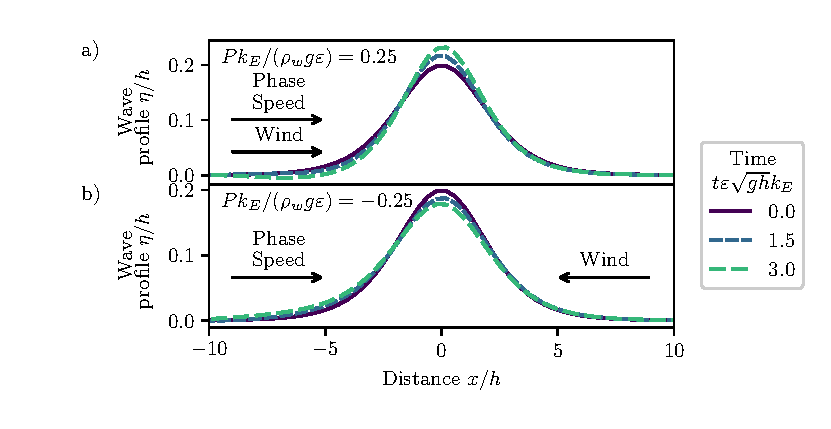
\includegraphics{Snapshots-Positive-Negative-Production.eps}
  \caption{
    Evolution of a solitary wave profile under
    \subref{fig:snapshots_solitary:a}
    onshore and
    \subref{fig:snapshots_solitary:b}
    offshore Jeffreys forcing in a frame co-moving with the unforced
    solitary wave speed.
    The non-dimension wave height $\eta/h$ is plotted for
    non-dimension distance $-10 \le x/h \le 10$.
    Results are shown for $\epsilon=0.1$, $\mu_E = 0.6$ and $\abs{P
    k_E/(\rho_w g \epsilon)} = 0.25$ non-dimension slow times $t'_1 = t
    \epsilon \sqrt{gh} k_E = 0$, $1.5$ and $3$, as indicated in the
    legend.
    The arrows denote the direction of wave propagation (phase speed) or
    wind direction.
  }\label{fig:snapshots_solitary}
\end{figure}

The wave profile $\eta/h$ snapshots in \cref{fig:snapshots_solitary}
qualitatively show how the wave shape evolves over non-dimension time
$t'_1 = t \epsilon \sqrt{g h} k_E$ when plotted against the
non-dimension distance $x/h$ in a frame co-moving with the unforced
solitary wave speed.
Despite the wave starting from a symmetric, solitary-wave initial
condition, the wind induces a horizontal asymmetry in the wave shape,
particularly on the rear face ($x<0$) of the wave.
Namely, the offshore wind (\cref{fig:snapshots_solitary:b}) raises the
rear base of the wave (near $x/h = -5$) relative to its initial profile
(purple line), but an onshore wind (\cref{fig:snapshots_solitary:a})
depresses it, even forming a small depression below the still water
level near $x/h = -6$ at $t\epsilon \sqrt{gh} k_E=3$ (green line).
Additionally, the onshore wind (\cref{fig:snapshots_solitary:a})
increases the slope of the wave with time while the offshore wind
(\cref{fig:snapshots_solitary:b}) decreases it, though the windward side
of the wave becomes steeper than the leeward side for both winds (up to
\SI{8}{\percent} steeper for the time period shown).
Finally, the onshore wind (\cref{fig:snapshots_solitary:a}) generates
wave growth, apparent at the wave crest $x=0$, while the onshore wind
(\cref{fig:snapshots_solitary:b}) causes the wave to decay.

\begin{figure}
  \centering
  { % Put \phantomsubcaption in their own group to prevent it from
    % affecting the main figure's numbering
    \phantomsubcaption{}\label{fig:statistics_solitary:a}
    \phantomsubcaption{}\label{fig:statistics_solitary:b}
    \phantomsubcaption{}\label{fig:statistics_solitary:c}
  }
  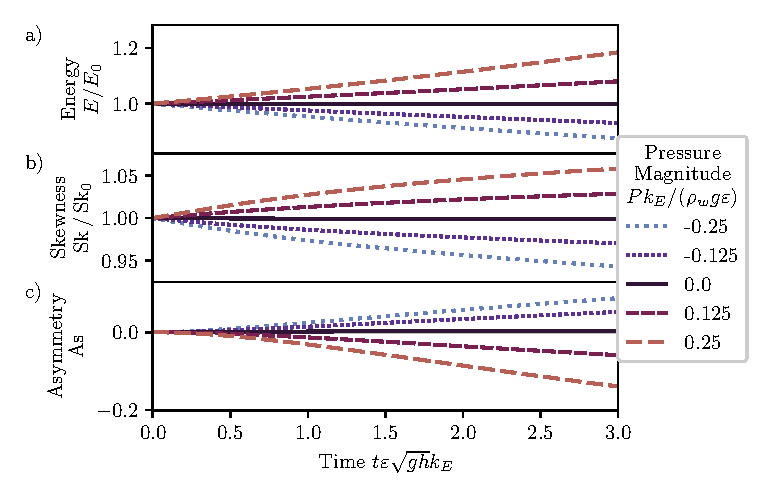
\includegraphics{Skew-Asymm-Production.eps}
  \caption{
    Shape statistics of a solitary profile under onshore and offshore
    Jeffreys forcing are shown for non-dimension slow time $t'_1 = t
    \epsilon \sqrt{gh} k_E = \numrange{0}{3}$.
    The
    \subref{fig:statistics_solitary:a}
    height,
    \subref{fig:statistics_solitary:b}
    skewness normalized by the initial time and
    \subref{fig:statistics_solitary:c}
    asymmetry are defined in
    \cref{eq:height_def,eq:shape_stats_def}.
    Results are shown for $\epsilon=0.1$, $\mu_E = 0.6$ and $P
    k_E/(\rho_w g \epsilon) = 0$, $\pm 0.125$ and $\pm 0.25$, as
    indicated in the legend.
    The solid black line corresponds to the unforced case, $P = 0$, and
    shows no growth or asymmetry and a constant, positive skewness.
  }\label{fig:statistics_solitary}
\end{figure}

To quantify the effect of wind on wave shape,
\cref{fig:statistics_solitary} shows shape statistics as functions of
the non-dimension slow time $t'_1 = t \epsilon \sqrt{g h} k_E$ for
onshore to offshore wind with $P k_E/(\rho_w g \epsilon)$ varying
between $\pm 0.25$.
We plot all cases for initial steepness $\epsilon = 0.1$ up to slow time
$t \epsilon \sqrt{g h} k_E = 3$, corresponding to $3/\epsilon = 30$
wave-crossing times, $\sqrt{gh} k_E$.
The height (\cref{fig:statistics_solitary:a}) begins at $H_0/h = 2
\epsilon = 0.2$ and shows an asymmetry in growth/decay rates: the
onshore wind ($P>0$) causes accelerating wave growth while the offshore
wind ($P<0$) causes decay which slows over time.
We can even see this qualitatively in the accelerating crest growth
(\cref{fig:snapshots_solitary:a}) and decelerating crest decay
(\cref{fig:snapshots_solitary:b}) at $x=0$ of
\cref{fig:snapshots_solitary}.

We can also quantify wave shape by the third-order moments, skewness
(\cref{fig:statistics_solitary:b}) and asymmetry
(\cref{fig:statistics_solitary:c}).
The onshore (offshore) causes the wave to become more (less) skewed over
time.
The skewness is nearly symmetric with respect to $\pm P$ about one.
The initial profile has zero asymmetry, and the unforced case
$P=0$ maintains zero asymmetry over time.
However, the onshore wind causes a backwards tilt and negative
asymmetry, while the offshore wind increases the asymmetry causing the
wave to tilt forwards, as seen in \cref{fig:snapshots_solitary}.
Notice that $\abs{\As}$ is larger for onshore winds than offshore winds.
The definitions of the skewness and asymmetry are insensitive to scaling
of the waveform $\eta \to \lambda \eta$, so this effect is not simply
caused by the wave's growth under an onshore wind.
Instead, the rear face of the wave shows larger deviations from the
unforced Stokes wave than the front face
(\cref{fig:snapshots_solitary}).
These deviations contribute strongly to the asymmetry, and the onshore
wind (\cref{fig:snapshots_solitary:a}) causes larger changes to the rear
face, and hence asymmetry, than offshore wind
(\cref{fig:snapshots_solitary:a}) does.
Though this analysis focuses on solitary waves, we also investigated the
effect of wind on periodic waves using the cnoidal-wave KdV solutions as
initial conditions.
The wind-induced pressure induced shape statistics were qualitatively
similar to those derived for solitary waves, so they are not shown here
for brevity.

\section{\label{sec:discussion} Discussion}

\subsection{\label{sec:press_mag} Wind Speed Estimation}
In \cref{sec:nondim}, we chose to non-dimensionalize the pressure as $P
k_E/(\rho_w g) = \order{\epsilon}$.
Now, we estimate the wind speed associated with such a pressure
to show that this choice is reasonable.
First we need relate the surface pressure to changes in the wave energy $E$,
\begin{equation}
  E \coloneqq \rho_w g \int_{-\infty}^{\infty} {\eta}_0^2 \dd{x} \,.
\end{equation}
We we can approximate the relationship between $E$ and $P$ starting from
the non-dimensional (denoted by primes) KdV-Burgers equation
\cref{eq:kdv_burgers} by using the standard procedure
\citep[\eg][]{mei2005nonlinear} of multiplying by $\eta'_0$ and
integrating from $x'=-\infty$ to $\infty$ to obtain
\begin{equation}
  \pdv{t'_1} \int_{-\infty}^{\infty} {\eta'}_0^2 \dd{x}
  = \int_{-\infty}^{\infty} P' \pqty{\pdv{\eta'_0}{x'}}^2
  \dd{x} \,.
\end{equation}
The left integral is the non-dimensional energy, so redimensionalizing
and converting back to the full time $t$ gives the energy growth rate
$\gamma$,
\begin{equation}
  \frac{\gamma}{c k_E} \coloneqq
  \frac{1}{c k_E E} \pdv{E}{t}
  = \frac{P k_E}{\rho_w g} \frac{\langle (\partial_x \eta)^2 \rangle}
    {\langle (k_E \eta)^2 \rangle}
  = \frac{1}{5} \frac{P k_E}{\rho_w g}
  \,.
  \label{eq:gamma_vs_P_solitary}
\end{equation}
In the final equation, we evaluated the growth rate for the initial
solitary wave profile (\cf{} \cref{sec:initial}).
Alternatively, we can numerically fit the energy growth rate to
\begin{equation}
  E \propto \frac{1}{1 - \gamma t}
  \qq{with}
  \gamma \coloneqq b \bqty{\frac{P k_E}{\rho_w g}} c k_E
  \,,
  \label{eq:actual_energy}
\end{equation}
with the phase speed $c = \sqrt{gh}$ and $b = \num{0.1992 \pm 0.0001}$.
\Cref{eq:actual_energy} has the same functional form and approximately
the same analytic growth rate $\gamma = (2/15) (P k_E/\rho_w g
\epsilon) ck$ as derived, for example, by \citet{zdyrski2019effects}
with a secondary multiple scales approximation of the KdV-Burgers
equation acting on a solitary wave.
Note that this expressions for $\gamma$ is consistent with the
KdV-Burgers approximation \cref{eq:gamma_vs_P_solitary} for small times
$\gamma t \ll 1$.
Furthermore, both expressions for $\gamma$ are consistent with the
observation in \cref{fig:snapshots_solitary,fig:statistics_solitary}
that the energy (and height) change accelerates for $P>0$ but
decelerates for $P<0$.

Additionally, \citet{jeffreys1925formation} theory relates the growth
rate of periodic waves to the wind speed $U_z$ (the subscript giving the
measurement height $z$) as
\begin{equation}
  \frac{\gamma}{c k} = S_z \frac{\rho_a}{\rho_w}
    \pqty{\frac{U_z}{c}-1} \abs{\frac{U_z}{c}-1} \,,
  \label{eq:gamma_vs_u_jeffreys}
\end{equation}
with $S_z$ a small, non-dimensional sheltering parameter potentially
dependent on the $\epsilon$, $\mu_E$ and $U_z/c$.
Combining this with \cref{eq:gamma_vs_P_solitary} gives
\begin{equation}
  U_z = c \pqty{1 \pm \sqrt{\frac{1}{5} \abs{\frac{P k_E}{\rho_w g}}
    \frac{\rho_w}{\rho_a} \frac{1}{S_z}}} \,.
  \label{eq:U_vs_P}
\end{equation}
Here, the $\pm$ corresponds to onshore ($+$) or offshore ($-$) winds.
Note that changing the wind direction (\ie{} sign of $Pk_E/(\rho_w g)$,
or $\pm$ sign) while holding the surface pressure magnitude
$\abs{Pk_E/(\rho_w g)}$ constant means $\abs{U_z}$ onshore will be
larger than $\abs{U_z}$ offshore.

We can evaluate \cref{eq:U_vs_P} for the parameters used in
\cref{sec:results} ($\epsilon=0.1$, $\mu_E = 0.6$, $Pk/(\rho_w g
\epsilon) = 0.25$).
\Citet{donelan2006wave} provides a parameterization of $S_z$ for
shallow-water waves that depends on airflow separation (and a separation
criterion): $S_{\lambda/2} = 4.91 \epsilon \sqrt{\mu}$ for non-separated
flow (such as ours), with $U_z$ measured at $z=\lambda/2$ and $\mu
\coloneqq (kh)^2$.
While \citet{donelan2006wave} measured this parameterization for
periodic waves, we will assume it holds approximately for solitary waves
and choose $ \lambda = 2 \pi/k_E =
\SI{20}{\meter}$ to directly give the wind speed at $z = \lambda/2 =
\SI{10}{\meter}$.
This choice corresponds to a depth of $h = \SI{2.5}{\meter}$ and initial
wave height $H_0 = \SI{0.5}{\meter}$ and yields a wind speed of $U_{10}
= \SI{21}{\meter\per\second}$, a reasonable wind speed for strongly
forced shallow-water waves.

\subsection{\label{sec:physical_reason} Physical Interpretation}
In \cref{sec:results}, we noted that the rear face ($x<0$) of the waves
in \cref{fig:snapshots_solitary} showed marked shape differences between
onshore and offshore wind, while the front faces ($x>0$) were rather
similar.
We can understand this by considering the fluid velocity in the
co-moving frame of \cref{fig:snapshots_solitary}.
The surface pressure $p \propto \partial_x \eta$ only does work
close to the wave where $\partial_x \eta$ is significant.
In front of the wave, the slope is small so the surface pressure acting
on the wave approaching the front face of the wave is negligible and
causes little shape change.
The front face of the wave has a large slope and thus large pressure,
causing the onshore (offshore) wind to begin adding (removing) energy
from the water flow.
However, the wave slope, and hence surface pressure, are large near the
front and rear wave face.
Similarly, the rear face of the wave also adds (removes) energy for
onshore (offshore) wind.
Thus, the wind has done work on the water leaving the rear face of the
wave.
The additional kinetic energy from the onshore wind causes the
downward-moving water to overshoot $z=0$ at the rear base of the wave,
leading to the depression seen in \cref{fig:snapshots_solitary:a}.
Conversely, the offshore wind does negative work, and the decreased
kinetic energy delays the flow's return to the still water level in
\cref{fig:snapshots_solitary:b}.
As discussed in \cref{sec:results}, this discrepancy between the front
and rear wave faces is responsible for much of the variation between
onshore asymmetry and offshore asymmetry in
\cref{fig:statistics_solitary:c}.

\subsection{Comparison to Intermediate and Deep Water}
Here, we have coupled wind to waves in shallow water.
A previous study \citep{zdyrski2020wind} instead studied the effect of
wind on Stokes-like waves in intermediate to deep water.
However, qualitative agreement is still found between these two studies.
\Cref{fig:statistics_solitary} shows that, for a fixed time $t \neq 0$,
the asymmetry increases as the pressure $P$ increases.
\Figname{} 4(a) of \citet{zdyrski2020wind} displayed a similar trend for
the corresponding Jeffreys pressure profile with positive (negative)
pressure increasing (decreasing) the asymmetry.
In addition to the Jeffreys-type forcing employed here,
\citet{zdyrski2020wind} also utilized a Generalized Miles (GM)-type
wherein the pressure was proportional to $\eta$ shifted by a distance
parameter $\psi_P/k$ which is only suitable for periodic waves.
However, results for GM forcings were not included here since the GM
forcing gives rise to a nonlocal KdV equation and produces unphysical
effects such as the growth of higher harmonics under offshore winds.
Finally, no appropriate experiments of wind and shallow-water wave shape
exist to compare to with our results.

\section{Conclusion}
Prior results~\citep{zdyrski2020wind} in intermediate and deep water
demonstrated that wind, acting though an $\eta$-dependent surface
pressure, can generate shape changes that become more pronounced in
shallow water.
This motivated the current work which used a multiple scales analysis to
couple weak wind with small, shallow-water waves, \ie{} $H_0/h \sim (k_E
h)^2 \sim P k/(\rho_w g) \ll 1$.
This derivation produced a KdV-Burgers equation governing the wave
profile $\eta$.
We utilized a symmetric solitary wave satisfying the unforced KdV
equation as our initial condition.
A third-order Runge Kutta solver determined the time-evolution of the
surface profile, and we extracted height, skewness and asymmetry as
functions of time and pressure magnitude.
For onshore wind (positive $P$), wave height and skewness increased with
time while asymmetry decreased, with offshore wind producing opposite
effects.
Furthermore, these effects were enhance for strong pressures, reducing
to the unforced case for $P=0$.
The shape statistics found here show qualitative agreement with the
results in intermediate and deep water, and future work on periodic
shallow-water waves would allow a direct, quantitative comparison with
the periodic deep-water waves.
Declaration of Interests. The authors report no conflict of interest.

\appendix

% Bibliography
\bibliographystyle{jfm}
\bibliography{references}

\end{document}
